\documentclass[11pt]{exam}
\newcommand{\myname}{Nishant Aswani}
\newcommand{\mynetid}{nsa325}
\newcommand{\myemail}{nsa325@nyu.edu}
\newcommand{\myhwtype}{Homework}
%%%%%%%%%%%%%%%%%%%%%%%%%%%%%%%%
\newcommand{\myhwnum}{8}
%%%%%%%%%%%%%%%%%%%%%%%%%%%%%%%%
\newcommand{\mycoursenumber}{ENGR-UH 3511}
\newcommand{\myclassname}{Computer Organization and Architecture}

\newcommand{\cc}[1]{\texttt{#1}}

% Prefix for numedquestion's
\newcommand{\questiontype}{Question}

% Use this if your "written" questions are all under one section
% For example, if the homework handout has Section 5: Written Questions
% and all questions are 5.1, 5.2, 5.3, etc. set this to 5
% Use for 0 no prefix. Redefine as needed per-question.
\newcommand{\writtensection}{0}

\usepackage{amsmath, amsfonts, amsthm, amssymb}  % Some math symbols
\usepackage{enumerate}
\usepackage{enumitem}
\usepackage{graphicx}
\usepackage{hyperref}
\usepackage[all]{xy}
\usepackage{wrapfig}
\usepackage{fancyvrb}
\usepackage[T1]{fontenc}
\usepackage{listings}
\lstset{
  basicstyle=\ttfamily,
  mathescape
}
\usepackage{fancyhdr}
\usepackage{booktabs}
\usepackage{makecell}
\usepackage{hhline}
\usepackage[utf8]{inputenc}

\usepackage[sorting=none,style=numeric]{biblatex}
\addbibresource{refs.bib}

% \usepackage{centernot}
\usepackage{mathtools}
\DeclarePairedDelimiter{\ceil}{\lceil}{\rceil}
\DeclarePairedDelimiter{\floor}{\lfloor}{\rfloor}
\DeclarePairedDelimiter{\card}{\vert}{\vert}

% Uncomment the following line to get Solarized-themed source listings
% You will have had to already installed the solarized-light package
% https://github.com/jez/latex-solarized
%
%\usepackage{solarized-light}

\setlength{\parindent}{0pt}
\setlength{\parskip}{5pt plus 1pt}
\pagestyle{empty}

\def\indented#1{\list{}{}\item[]}
\let\indented=\endlist

\newcounter{questionCounter}
\newcounter{partCounter}[questionCounter]

\newenvironment{namedquestion}[1]{%
    \addtocounter{questionCounter}{1}%
    \setcounter{partCounter}{0}%
    \vspace{.2in}%
        \noindent{\bf #1}%
    \vspace{0.3em} \hrule \vspace{.1in}%
}{}

\newenvironment{numedquestion}[0]{%
	\stepcounter{questionCounter}%
    \vspace{.2in}%
        \ifx\writtensection\undefined
        \noindent{\bf \questiontype \; \arabic{questionCounter}. }%
        \else
          \if\writtensection0
          \noindent{\bf \questiontype \; \arabic{questionCounter}. }%
          \else
          \noindent{\bf \questiontype \; \writtensection.\arabic{questionCounter} }%
        \fi
    \vspace{0.3em} \hrule \vspace{.1in}%
}{}

\newenvironment{alphaparts}[0]{%
  \begin{enumerate}[label=\textbf{(\alph*)}]
}{\end{enumerate}}

\newenvironment{arabicparts}[0]{%
  \begin{enumerate}[label=\textbf{\arabic{questionCounter}.\arabic*})]
}{\end{enumerate}}

\newenvironment{questionpart}[0]{%
  \item
}{}

\newcommand{\answerbox}[1]{
\begin{framed}
\vspace{#1}
\end{framed}}

\pagestyle{head}

\headrule
\header{\textbf{NYU Abu Dhabi}}%
{\textbf{}}%
{\textbf{Division of Engineering}}

\pagestyle{head}

\begin{document}

\begin{center}
  
\includegraphics[scale=0.15]{etc/NYUAD-alt-logo.jpg}
\end{center}

{\vspace{1.5em}}

\begin{center}
    \Huge{\textbf{\mycoursenumber}}\\
    {\vspace{0.5em}}
    \Huge{\textbf{\myclassname}}
\end{center}

{\vspace{10em}}

\begin{center}
  \begin{tabular}{|rp{5.0cm}lll|}
    \hline
    &  &  &  & \\
    &  &  &  & \\
    \Large{\textbf{Name:}} & \Large{\myname}
    
    \  &  &  & \\
    \Large{\textbf{Net ID:}} & \Large{\mynetid}
    
    \  &  &  & \\
    \Large{\textbf{Assignment Title:}} & \Large{\myhwtype{} \myhwnum}
    
    \
    
    \  &  &  & \\
    \hline
  \end{tabular}
\end{center}

\

{\newpage}


\thispagestyle{plain}
\begin{center}
  {\Large \mycoursenumber{} \myhwtype{} \myhwnum} \\
  \myname{} (\myemail{}) \\
  \today
\end{center}

\setcounter{questionCounter}{0}

\begin{namedquestion}{Problem 1.6 Case Study}

General-purpose processes are optimized for general-purpose computing. That is, they are optimized for behavior that is gener-ally found across a large number of applications. However, once the domain is restricted somewhat, the behavior that is found across a large number of the target applications may be different from general-purpose applications. One such appli-cation is deep learning or neural networks. Deep learning can be applied to many different applications, but the fundamental building block of inference—using the learned information to make decisions—is the same across them all. Inference operations are largely parallel, so they are currently performed on graphics proces-sing units, which are specialized more toward this type of computation, and not to inference in particular. In a quest for more performance per watt, Google has cre-ated a custom chip using tensor processing units to accelerate inference operations in deep learning. 1 This approach can be used for speech recognition and image recognition, for example. This problem explores the trade-offs between this pro-cess, a general-purpose processor (Haswell E5-2699 v3) and a GPU (NVIDIA K80), in terms of performance and cooling. If heat is not removed from the com-puter efficiently, the fans will blow hot air back onto the computer, not cold air. Note: The differences are more than processor—on-chip memory and DRAM also come into play. Therefore statistics are at a system level, not a chip level.\\

\begingroup
    \centering
    \medskip
    %width=\columnwidth
    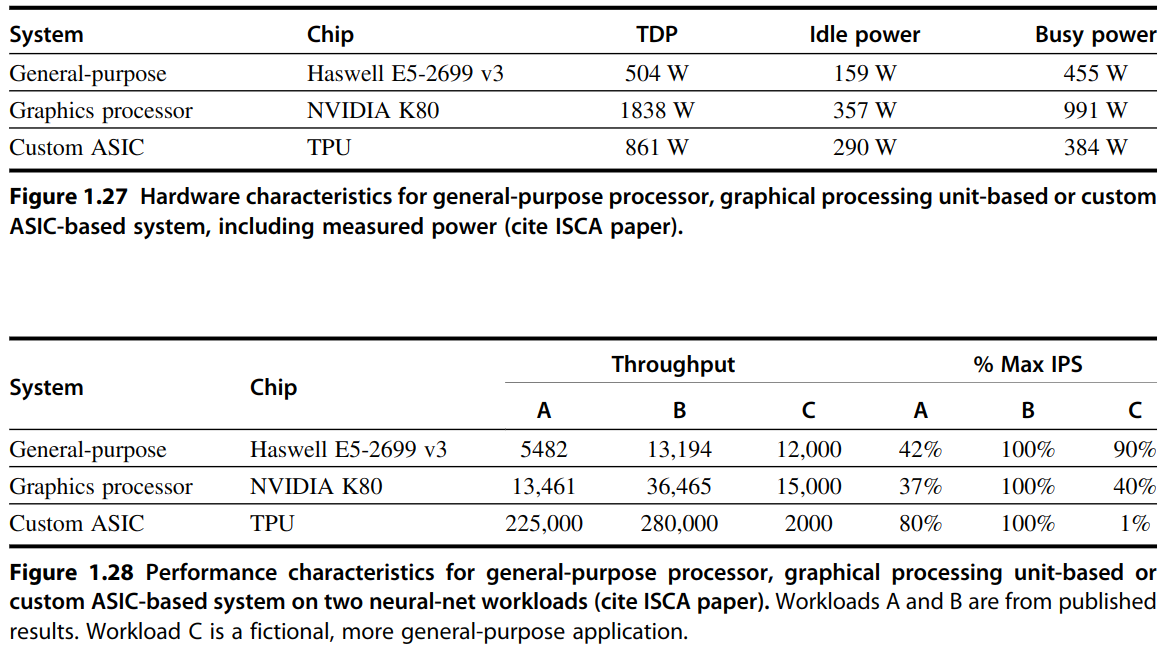
\includegraphics[width=\columnwidth]{Homework-Tex/img/16tb.png}
    \medskip
\endgroup

\end{namedquestion}

\newpage

\begin{namedquestion}{Problem 1.6A}

\textit{Google’s data center spends 70\% of its time on workload A and 30\% of its time on workload B when running GPUs, what is the speedup of the TPU system over the GPU system?}\\

\begin{equation}
    \begin{split}
        \text{Speedup} &= \frac{Performance_{TPU}}{Performance_{GPU}} =  \frac{Exec Time_{GPU}}{Exec Time_{TPU}}\\
    \end{split}
\end{equation}


\begin{equation}
    \begin{split}
        \text{Speedup Workload A} &= \frac{225,000}{13,461} = 16.7 \\
        \\
        \text{Speedup Workload B} &= \frac{280,000}{36,465} = 7.7 \\
    \end{split}
\end{equation}

\begin{equation}
    \begin{split}
        \text{Speedup} &= \frac{1}{(1 - Frac_{Enhanced}) + \frac{Frac_{Enhanced}}{Speedup_{Enhanced}}}\\
        \\
        &= \frac{1}{(1 - 1) + (\frac{0.7}{16.7} + \frac{0.3}{7.7})} \\
        \\
        &= \frac{1}{\frac{0.7}{16.7} + \frac{0.3}{7.7}}\\ 
        \\
        \textbf{Speedup} &= \textbf{12.36}
    \end{split}
\end{equation}

\newpage

\begin{namedquestion}{Problem 1.6B}
\end{namedquestion}

\textit{Google’s data center spends 70\% of its time on workload A and 30\% of its time on workload B when running GPUs, what percentage of Max IPS does it achieve for each of the three systems?}\\


\begin{equation}
    \begin{split}
        \text{Max IPS \% for CPU} &= 0.7(0.42) + 0.3(1) = 0.594 \\
        \\
        \text{Max IPS \% for GPU} &= 0.7(0.37) + 0.3(1) = 0.559 \\
        \\
        \text{Max IPS \% for TPU} &= 0.7(0.80) + 0.3(1) = 0.860\\
    \end{split}
\end{equation}


\textbf{
General Purpose Unit => 59.4\% \\
GPU => 55.9\% \\
TPU => 86.0\% \\

}

\end{namedquestion}

\begin{namedquestion}{Problem 1.6C}
\textit{Building on (b), assuming that the power scales linearly from idle to busy power as IPS grows from 0\% to 100\%, what is the performance per watt of the TPU system over the GPU system?}\\


The graph below shows the power used at the determined IPS:

\begingroup
    \centering
    \medskip
    %width=\columnwidth
    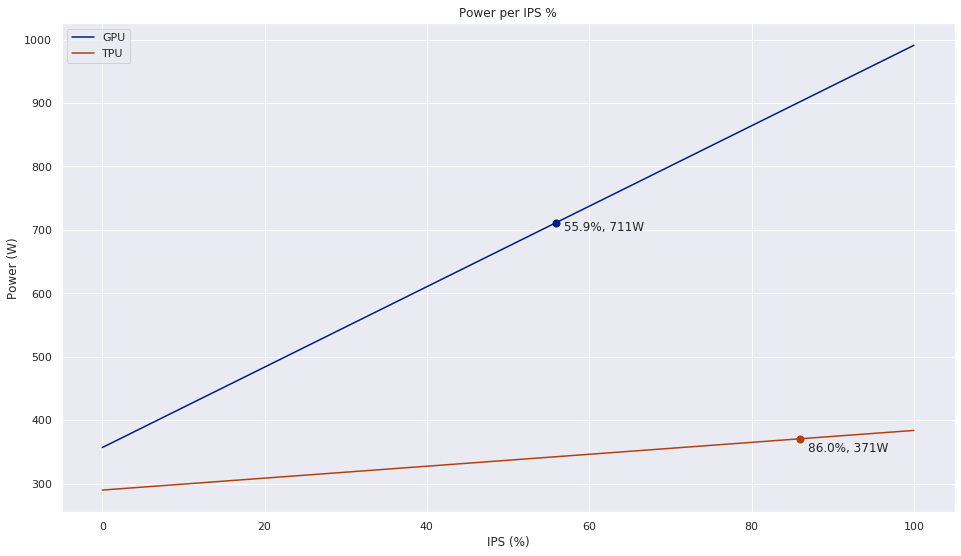
\includegraphics[width=\columnwidth]{Homework-Tex/img/power.png}
    \medskip
\endgroup

The power consumption for the hardware can be modeled using:

\begin{equation}
    \begin{split}
        \text{Power GPU} = \frac{991-357}{100}x_{1} - 357 = \frac{991-357}{100}*55.9 - 357 = 711W\\
        \\
        \text{Power TPU} = \frac{384-290}{100}x_{2} - 290 = \frac{384-290}{100}*86.0 - 290 = 371W\\
        \\
    \end{split}
\end{equation}

\begingroup
    \medskip
    \centering
    \def\arraystretch{1.5}
        \begin{tabular}{lcc}
            \toprule
            Weighted IPS & Power(W) & Instructions per Watt Second\\
            \midrule
            0.559*13,461 = 7,376 & 711 & 10.37\\
            0.860*280,000 = 240,800 & 371 & 649\\
            \bottomrule
        \end{tabular}
    \label{fig:noOptimization}
    \medskip
\endgroup

\\

\textbf{The performance per watt is $\frac{649}{10.37}$ = 62.58 greater in the TPU than in the GPU}

\end{namedquestion}

\begin{namedquestion}{Problem 1.6D}
\textit{
 If another data center spends 40\% of its time on workload A, 10\% of its time on workload B, and 50\% of its time on workload C, what are the speedups of the GPU and TPU systems over the general-purpose system?} \\

Calculating speedup with TPU

\begin{equation}
    \begin{split}
        \text{Speedup Workload A} &= \frac{225,000}{5,482} = 41.04\\
        \\
        \text{Speedup Workload B} &= \frac{280,000}{13,194} = 21.22 \\
        \\
        \text{Speedup Workload C} &= \frac{2,000}{12,000} = 0.17 \\
    \end{split}
\end{equation}

\begin{equation}
    \begin{split}
        \text{Speedup TPU} &= \frac{1}{(1 - Frac_{Enhanced}) + \frac{Frac_{Enhanced}}{Speedup_{Enhanced}}}\\
        \\
        &= \frac{1}{(1 - 1) + (\frac{0.4}{41.04} + \frac{0.1}{21.22} + \frac{0.5}{0.17})} \\
        \\
        &= \frac{1}{(\frac{0.4}{41.04} + \frac{0.1}{21.22} + \frac{0.5}{0.17})} \\
        \\
        \textbf{Speedup TPU} &= \textbf{0.33}
    \end{split}
\end{equation}

\\

Calculating speedup with GPU

\begin{equation}
    \begin{split}
        \text{Speedup Workload A} &= \frac{13,461}{5,482} = 2.46\\
        \\
        \text{Speedup Workload B} &= \frac{36,465}{13,194} = 2.76\\
        \\
        \text{Speedup Workload C} &= \frac{15,000}{12,000} = 1.25\\
    \end{split}
\end{equation}

\begin{equation}
    \begin{split}
        \text{Speedup GPU} &= \frac{1}{(1 - Frac_{Enhanced}) + \frac{Frac_{Enhanced}}{Speedup_{Enhanced}}}\\
        \\
        &= \frac{1}{(1 - 1) + (\frac{0.4}{2.46} + \frac{0.1}{2.76} + \frac{0.5}{1.25})} \\
        \\
        &= \frac{1}{(\frac{0.4}{2.46} + \frac{0.1}{2.76} + \frac{0.5}{1.25})} \\
        \\
        \textbf{Speedup GPU} &= \textbf{1.67}
    \end{split}
\end{equation}

\end{namedquestion}

\newpage

\begin{namedquestion}{Problem 1.6E}

\textit{A cooling door for a rack costs \$4000 and dissipates 14 kW (into the room; additional cost is required to get it out of the room). How many Haswell-, NVIDIA-, or Tensor-based servers can you cool with one cooling door, assuming TDP in Figures 1.27 and 1.28? }



\begin{equation}
    \begin{split}
        \text{No. of Haswell E5-2699 v3 Cooled} &= \frac{14000}{504} = 27 \text{ units} \\
        \\
        \text{No. of NVIDIA K80 Cooled} &= \frac{14000}{1838} = 7 \text{ units} \\
        \\
        \text{No. of TPUs Cooled} &= \frac{14000}{861} = 16 \text{ units} \\
    \end{split}
\end{equation}

\end{namedquestion}

\begin{namedquestion}{Problem 1.6F}
\textit{Typical server farms can dissipate a maximum of 200 W per square foot. Given that a server rack requires 11 square feet (including front and back clearance), how many servers from part (e) can be placed on a single rack, and how many cooling doors are required?}

\begin{equation}
    \begin{split}
        \frac{\text{Haswell Power}}{\text{server rack space}} & <= \text{200 W/sqft}\\
        \\
        \frac{H * 504}{11} & <= 200\\
        \\
        H & <= \frac{200*11}{504}\\
        \\
        \textbf{H} & <= \textbf{4 units}
    \end{split}
\end{equation}

\begin{equation}
    \begin{split}
        \frac{\text{Nvidia Power}}{\text{server rack space}} & <= \text{200 W/sqft}\\
        \\
        \frac{N * 1838}{11} & <= 200\\
        \\
        N & <= \frac{200*11}{1838}\\
        \\
        \textbf{N} & <= \textbf{1 unit}
    \end{split}
\end{equation}

\begin{equation}
    \begin{split}
        \frac{\text{TPU Power}}{\text{server rack space}} & <= \text{200 W/sqft}\\
        \\
        \frac{T * 861}{11} & <= 200\\
        \\
        T & <= \frac{200*11}{861}\\
        \\
        \textbf{T} & <= \textbf{2 units}
    \end{split}
\end{equation}
\\

\textbf{In all cases, we will only need 1 cooling door per server rack.}


\end{namedquestion}


\printbibliography

\end{document}

% \begingroup
%     \medskip
%     \centering
%     \def\arraystretch{1.5}
%         \begin{tabular}{cc}
%             \toprule
%             RAW hazard & stall cycles\\
%             \midrule
%             Ex to 1st & 2\\
%             Mem to 1st & 2\\
%             Ex to 2nd & 1\\
%             Mem to 2nd & 1\\
%             Ex to 1st and Mem to 2nd & 2\\
%             \bottomrule
%         \end{tabular}
%     \label{fig:c2table2}
%     \medskip
% \endgroup


